\chapter{Testplan}
To determine requirement, structural, and architectural coverage of our
product, software testing has been performed. The tests are formalized
to make it easier to agree on the coverage between the customer,
maintainers, and us. The results and process is documented in this
chapter.

\section{Testing Strategy Overview}
It is common practise to structure tests in three categories. This way,
tests can be communicated to developers, stakeholders, and high-level
non-technical users. 
Following is our interpretation of each category.
\subsection{Unit Testing}
Unit testing is the process of testing program components individually.
The tests invoke methods and structures in the code using different
input parameters. These are usually written before or
immediately after a module is completed. This way, it is easier to
assert that the module does what it is intended. Each test case is
independent from each other, so several people can write test cases
simultaneously without having to worry about dependencies.

\subsection{Integration Testing}
In development, many features are bundled into different components. The
components are then joined together to form a system. The interfaces to 
each of these components, and how they communicate with each other, are tested during Integration
testing. The purpose is to ensure that
communication between the components is correct, and that the
components work as intended. It can be extensive if those responsible
for integration have to review the code in each component, so
integration testing abstract code away. If there are any errors, then
one will either review the unit tests or notify the author.

\subsection{System Testing}
System testing is a high-level test of the system. It is performed after
all of the integrated system parts have been tested and joined
together. System testing is a black box test, as anyone should be able
to perform the test without having any knowledge\ of the underlying
code. The purpose of system testing is to test if our system fulfills
the requirements in the requirement specification. This is important to
find out if we meet the expectations from the customer. 

\subsection{Acceptance Testing}
Acceptance tests are usually executed by the customers. They are written
after agreeing on the requirements specification for a delivery. The
tests are then verified by the customer. Once both the customer and
developers agree on the acceptance test, it will be possible to
formally agree on whether or not a delivery meets the given
requirements.

\subsection{Testing Coverage}
We wanted to provide complete test coverage, unfortunately, due to time contraints we where unable 
to achieve this goal. Thus, we needed to prioritize which components of the system were
most prone to error, and most important to test. The following were our
software assurance objectives:
\begin{itemize}
    \item Ensure that the system can be used by many users
    \item Ensure that the contest can be held without any error that would
critically impact the contest
\end{itemize}

Errors that solely impacted user experience were not prioritized to
test. The majority of these were intended to be found from debugging
the system. Since the developers would work closely with each other, 
we concluded that we would fix small errors in regression.
If our team had more members, or if we had been working in different
locations, this would have been a higher priority.

In most projects, testing is used to ensure requirements coverage. In
our case, however, with frequent customer-meetings and iterative
development, we have not had a strong need for this. The customer has
had access to prototypes of our solution and our source code. In order
to see that the product does as intended, they could simply try it out
for themselves.

As per our software assurance objectives, our largest focus has been
simulating the role of a contestant. To meet our objectives, we
intended to do a full coverage of all contestant scenarios. The
privileged users were believed to be technically experienced and
without intention to do harm. We still felt it was important to prevent
user errors, but our coverage was not as complete for these
usergroups.

Since we were developing a website that would feature many users,
developer testing alone could never simulate peak values for system
demand. We have relied on load testing, giving our Web
server a fixed amount of HTTP requests per second, hereafter RPS.\ What
pages were used in the simulation was determined by us. Thus, our
testing also extends to cover simulated peak values for high loads.

\section{Our Approach to Testing}
This section describes our approach to planning the different testing categories.
\subsection{Unit Testing}

We performed unit testing after the completion of a testable module. The
unit tests use the PyUnit framework, and is written by another person
than the one who produced the code for the module. I.e. if
person A makes module M, then person B will write the unit tests for
module M. The reason for having another person writing the test for a
module is because that will give more people insight in the code, and
make it easier to discover problems. The unit tests reside in the test.py 
file in each Django app.

\subsection{Integration Testing}
Each integration test will test a different interface. The interface is
defined as the connection between the different components in our
system. The pre- and post-condition sets the boundaries for the test.
Input and output is used to determine if the test produces the expected
output with a corresponding input. The motivation behind integration testing is that we
can determine whether a module has been successfully integrated. By
going through the accompanied tests made for the interfaces that
interact with the module


\subsection{System Testing}
Each separate test in the system test is linked to one or more of the
requirements from the requirements specification. This is to ensure 
that the system meets all the requirements set by the customer. The template for
system testing starts with specifying which function is being tested.
After that we say what the action/input should be, and what the
expected result is. The expected result needs to be achieved for the
test to be considered successful.


\subsection{Acceptance Testing}
The customer performed an acceptance test before each release of the
system, so they could confirm that we met the expected requirements.
The acceptance test was based on our system test, with the customer
executing the tasks in the system test. It was
approved when the customer was satisfied with how we implemented the
requirements.

\pagebreak
\section{Testing Results}
The results from our testing is presented in this section.

\subsection{Integration Test}
Each test has a unique identifier, name, pre/post-conditions and corresponding
input and output. An example is given in table~\ref{table:integrationTest}.

\begin{longtable}{|l|l|}
    \caption{Integration test for adding a sponsor} \label{table:integrationTest}\\
\hline
ID & IT-01\\\hline
Interface name & Add sponsor\\\hline
Pre-condtion & Contest is created\\\hline
Post-condition & Sponsor and image\\\hline
Input & Image, URL\\\hline
Output & Sponsor in contest\\\hline
\end{longtable}

In section X.X[12. Evaluation of testing methods] we explained why our
coverage by integration testing was not extensive. The written
integration tests are from our milestone M-03, First release, and only cover the
requirements that was necessary for that milestone. As such, we have
chosen to move all the integration tests to Appendix~\ref{appendix:integrationTest}

We formally agreed on what modules our system was made out of and their
interfaces. Figure~\ref{fig:componentDiagram} shows our view on the system as
per milestone M-03. In figure~\ref{fig:componentDiagram}, we have replaced
some default UML symbols and replaced them with the equivalent UML stereotype.
The explanations are given in table~\ref{table:component}. The integration
tests we did make are given in appendix~\ref{appendix:integrationTest}.

\begin{longtable}{|l|p{.6\textwidth}|}
    \caption{Symbiology for our UML component diagram} \label{table:component} \\
    \hline
    \textbf{UML stereotype} & \textbf{Function}\\
    \hline

    $<<$provides$>>$ & The component delivers the given functionality \\
    \hline

    $<<$requires$>>$& For the component to work it must have the given interface\\
        \hline
\end{longtable}

\begin{figure}[h!]
    \centering
    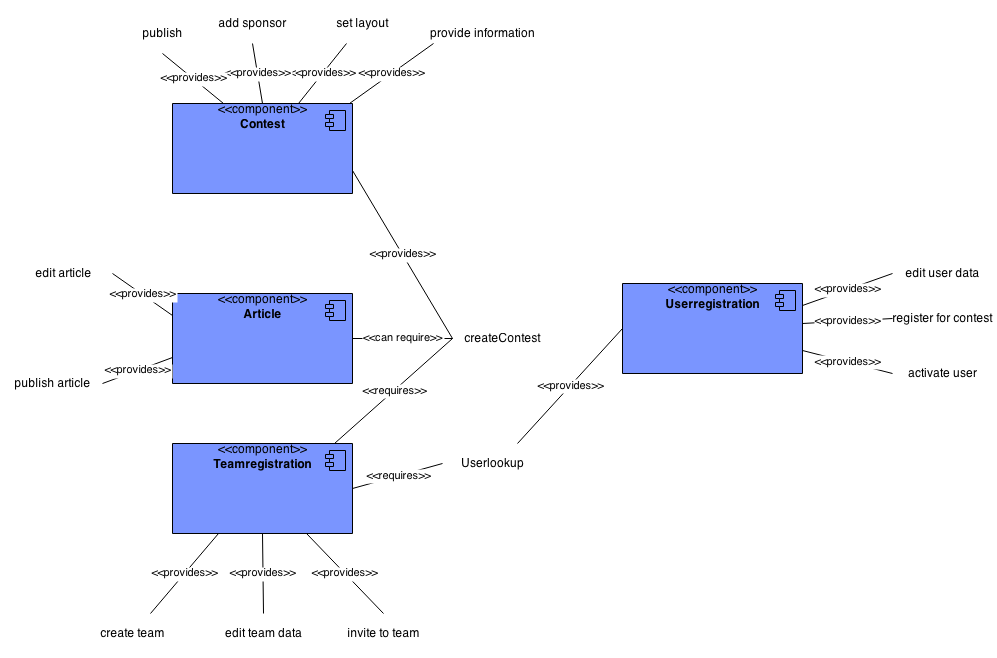
\includegraphics[width=.95\textwidth, height=.85\textheight]{UML_component.png}
    \caption{Diagram from milestone M-03. Each interface connection, especially
    ``createContest'' has been tested}
    \label{fig:componentDiagram}
\end{figure}

\pagebreak
\newpage
\section{System Test}
Our system tests cover all the functional requirements. All tests are
written as successive cases. This means that the tests do not cover
scenarios for how the system should respond when a user performs an
error or another external fault occurs. The complete listing is in
table~\ref{table:systest}.

\begin{longtable}{|l|p{3cm}|p{3cm}|p{3cm}|p{1.1cm}|l|}
\caption[table:systest]{System test} \label{table:systest}\\
\hline
\multicolumn{1}{|c|}{\textbf{ID}} &
\multicolumn{1}{c|}{\textbf{Function}} &
\multicolumn{1}{c|}{\textbf{Action/Input}} &
\multicolumn{1}{c|}{\textbf{Result}} &
\multicolumn{1}{c|}{\textbf{Req}} & 
\multicolumn{1}{c|}{\textbf{Pass/Fail}} \\
\hline 
\endfirsthead

\multicolumn{3}{c}%
{{\bfseries \tablename\ \thetable{} -- continued from previous page}} \\
\hline 
\multicolumn{1}{|c|}{\textbf{ID}} &
\multicolumn{1}{c|}{\textbf{Function}} &
\multicolumn{1}{c|}{\textbf{Action/Input}} &
\multicolumn{1}{c|}{\textbf{Result}} &
\multicolumn{1}{c|}{\textbf{Req}} & 
\multicolumn{1}{c|}{\textbf{Pass/Fail}} \\
\hline 
\endhead

ST-01 & Create a contest, and publish an article to that contest. Edit
article.Then, delete the contest. & Contest name, article text & Contest and
article is no longer publicly    available & FA-16, & PASS\\
\hline

ST-02 & As a contestant, create a team and invite contestants. Go to profile
page and see which team the contestant is amember of. Then, delete the team
& Team, contestants, contest & First contestant in team, then contestant not in
team & FE-01 FE-02 FE-04 FE-06 FC-04& PASS\\
\hline

ST-03 & Add custom css, specify custom settings, & Existing contest, css,
compiler flags, penaltysystem, maximum numbers of contestant, maximum number of
contestant per team & Contest with custom css and settings & FA-05 &
PASS\\
\hline 

ST-04 & Log in as admin, and enable all judges to createa contest. Then remove
and add a judge, by escalating and de-escalating privileges from contestant. &
Admin account, contestant account & Zero changes to system. &
FA-09 & PASS\\
\hline

ST-05 & Log in as judge, create a problem and upload cases. Upload different
solutions; one correct, one erroneous, and one that loops forever. After that,
modify the problem before deleting it.
& Problem, solutions, erroneous code, judge account &
Only the correct solution should give points. &
FJ-01 FJ-02 FJ-03 FJ-04 FJ-05 FJ-06 FJ-07&
PASS\\
\hline

ST-06 & Add two execution nodes with different compiler supports. Change both
nodes, such that they take each other's \ compiler setting. Then remove both
nodes. &
Compiler profiles, available nodes, production server, administrator account &
zero added nodes, no errors in execution & FA-12 FA-13 & PASS\\
\hline 

ST-07 & As a contestant, submit a question to the judge. As a judge, receive a
notification, and answer both the contestant and globally. &
Contestant, contest, question, answer &
All contestants should be able to see message, successful communication between
judge and contestant & FJ-08 & PASS\\
\hline

ST-08 & Create a contestant account. Activate the account via email, and change
the email. Ask for lost password on the new  email. &
Contest-data, emails & Activation data received on the email, and all links
word & FC-01 FC-02 & PASS\\
\hline
\end{longtable}

\pagebreak
\section{Non-functional testing}
% Our non-functional tests ensures non-functional requirements coverage
% and scenario correctness. Additionally, it defines acceptance criteria
% related to the performance of our solution.

The tests related to performance usually comes in pairs, a value and the
double of that value. This applies to the input and expected result.
This is to ensure that system performance does not scale down in a
non-linear way. E.g.\ if ``X''
transactions are processed and the server begins using swap memory
instead of RAM, this would mean that a high load would cause an
exponentially slower load rate for a high number of transactions.

Often, as mentioned in section X.X, we did
inspection tests. Thus, table~\ref{table:not} does not contain all tests that
are executed, and the table only covers the first 12 non-functional
requirements. The documented tests do, however, ensure some
requirements coverage.

\begin{longtable}{|p{4.3cm}|p{2.0cm}|l|p{3.8cm}|l|}
    \caption{System tests} \label{table:not} \\
\hline \multicolumn{1}{|c|}{\textbf{Case}} &
\multicolumn{1}{c|}{\textbf{Input}} &
\multicolumn{1}{c|}{\textbf{ID}} &
\multicolumn{1}{c|}{\textbf{Expected Result}} &
\multicolumn{1}{c|}{\textbf{Pass/Fail}} \\
\hline 
\endfirsthead

\multicolumn{3}{c}%
{{\bfseries \tablename\ \thetable{} -- continued from previous page}} \\
\hline \multicolumn{1}{|c|}{\textbf{Case}} &
\multicolumn{1}{c|}{\textbf{Input}} &
\multicolumn{1}{c|}{\textbf{ID}} &
\multicolumn{1}{c|}{\textbf{Expected Result}} &
\multicolumn{1}{c|}{\textbf{Pass/Fail}} \\
\hline 
\endhead

Adding 500 contestants & 500 users & NF-04 & Ability to add yet another & PASS\\
\hline
Adding 200 teams & 200 teams & NF-05 & Ability to add yet another & PASS\\
\hline
Adding 20 judges & 20 judges & NF-06 & Ability to add yet another &
PASS\\
\hline
Adding more than one admin &
$>$ 1 admin & NF-07 & Ability to add yet another & PASS\\
\hline
Upload a solution which is less than 50kB & Solution $>$ 50kB & NF-08 & Successful delivery & PASS\\
\hline
Upload a solution which is greater than 50kB & Solution $>$ 50kB & NF-08 & Error message & PASS\\
\hline
Gather some test persons not familiar with the system and have them use the
system as a contestant & System & NF-09 & They should be familiar with the
system after 5 minutes & FAIL\\
\hline
Gather some test persons not familiar with the system and have them use the
system as a judge & System & NF-11 & They should be familiar with the system
after 10 minutes & PASS\\
\hline
Gather some test persons not familiar with the system and have them use the
system as an admin & System & NF-10 & They should be familiar with the system
after 15 minutes & PASS\\
\hline
Page responsiveness with at least 5 RPS & HTTP GET and POST to all pages &
NF-01 & Response-time {\textless} 150 ms & FAIL\\
\hline
Page responsiveness with at least 10 RPS & HTTP GET and POST to all pages &
NF-01 & Response-time {\textless} 300 ms & FAIL\\
\hline
\end{longtable}

